\classheader{2018-10-15}
NEED TO FINISH ATLEAST 8 LECTURES FROM BEFORE
\begin{multicols}{2}
\begin{itemize}
	\item Modes of convergence; Slutsky's Theorem
	\item Asymptotic normality of MLEs
	\item Sufficiency
	\item Efficiency
\end{itemize}
\end{multicols}
\underline{4 Typical Modes of Convergence}
\begin{multicols}{2}
	\begin{enumerate}
	\item Convergence with probability 1
	\item Convergence in probability
	\item Convergence in $L^P$ (expectation)
	\item Convergence in distribution
\end{enumerate}
\end{multicols}
\begin{gather*}
	Y_n = g_n(X) = n \mathbbm{1}_{[0, \frac{1}{n} )} \qquad X \sim unif[0,1]\\
	Y_n \rightarrow y \quad \text{w.p. } 1 \quad \text{(away from zero) where } Y \equiv 0\\
	g_n(X) = n^2 \mathbbm{1}_{[0, \frac{1}{n} )}
\end{gather*}
\begin{enumerate}
	\item Here $Y_n \rightarrow 0$ w.p. 1
	\item $Y_n \rightarrow 0$ in probability
	\item $E[|Y_n|] = n$  so $Y_n \rightarrow Y$ in Expectation or $L^P$ for $p \geq 1$
\end{enumerate}
\underline{Exercise}: How can we construct a sequence $Y_n$ s.t. $Y_n \rightarrow 0$ in probability but $Y_n \cancel{\rightarrow} 0$ w.p. 1?\\
\begin{center}
	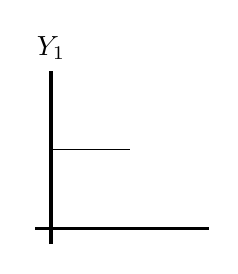
\begin{tikzpicture}[scale=2]
    		\draw[very thick,-] (-.1,0) -- (1,0);
		    \draw[very thick,-] (0,-.1) -- (0,1) node[above] {$Y_1$};

			\draw[-] (0,0.5) -- (0.5,0.5);			
			
\end{tikzpicture}
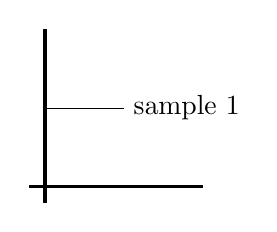
\begin{tikzpicture}[scale=2]
    		\draw[very thick,-] (-.1,0) -- (1,0);
		    \draw[very thick,-] (0,-.1) -- (0,1);

			\draw[-] (0,0.5) -- (0.5,0.5) node[right] {sample 1};			
			
\end{tikzpicture}
\end{center}
For each $\omega \in (0,1)$ the $Y_n$'s oscillate between 0 and 1, but the set of points at which $Y_n$ is non-zero shrinks in probability.\\
\textbf{Note:}
	If $Y_n \rightarrow Y$ with probability 1, then $Y_n \rightarrow Y$ in probability, but converse is not necessarily true.

\begin{theorem}
	Slutsky's Theorem: 
	\begin{enumerate}[label=\protect\circled{\arabic*}]
		\item Suppose $X_n \rightarrow X$ in distribution ($X_n \xrightarrow{d} X$), $Y_n \rightarrow Y$ in probability. Then $X_n + Y_n \xrightarrow{d} X + Y$
		\item If $X_n \xrightarrow{d} X$ and $Y_n \rightarrow c$ in probability: $X_n Y_n \xrightarrow{d} cX$
	\end{enumerate}
\end{theorem}
\underline{Why all this fuss?} Short answers: modes of convergence can be quire different!\\\\
Let's look at what happens to functions of random variables in particular:\\\\
Let $g: \mathbb{R} \rightarrow \mathbb{R}$ be smooth; and suppose $X_i \sim i.i.d. \quad f(x|\theta);$ \qquad $\mu = \mathbb{E}[X_i]; \quad Var(X_i) = \sigma^2 < \infty$\\\\
So $\bX$ is consistent for $\mu$. Further, by CLT $\Rightarrow$
\begin{gather*}
	\frac{\bX - \mu}{\frac{\sigma}{\sqrt{n}}} \underset{\text{approx}}{\sim} \mathcal{N}(0,1)\\
	\frac{\sqrt{n}}{\sigma} (\bX - \mu) \rightarrow \mathcal{N}(0,1)
\end{gather*}
How to understand approximatet/asymptotic behavior of $g(\bX)$? \textbf{Taylor expand} $g$ about $\mu$
\begin{equation*}
	g(x) \approx g(\mu) + g'(\mu) (x - \mu) + \frac{1}{2} g''(\mu) (x-\mu)^2
\end{equation*}
\underline{Taylor's theorem with remainder:}
\begin{equation*}
	g(x) \approx g(\mu) + g'(\mu) (x - \mu) + \frac{g''(Z)}{2!} (x-\mu)^2
\end{equation*}
where $Z$ is some point between $x$ \& $\mu$ 
\begin{align*}
	\Rightarrow g(\bX) - g(\mu) & = g'(\mu) (\bX - \mu) + \frac{g''(Z) (\bX -\mu)^2}{2!} \\
	\sqrt{n} \big( g(\bX) - g(\mu) \big) & = \underbrace{\boxed{\sqrt{n} g'(\mu) (\bX - \mu)}}_{\rightarrow \mathcal{N}(0, \text{some variance})} + \underbrace{\frac{\sqrt{n} g''(Z) (\bX -\mu)^2}{2!}}_{\circled{?}}
\end{align*}
\begin{align*}
	\circled{?} & = \sqrt{n} \underbrace{\frac{g''(Z)}{2!}}_{\substack{\text{suppose} \\ \text{we can bound} \\ \text{this piece}}} (\bX - \mu)^2\\
	\sqrt{n} (\bX - \mu)^2 & = \underbrace{\boxed{\sqrt{n}(\bX - \mu)}}_{\substack{\text{converging} \\ \text{ in distr} \\ \text{ to normal}}} \underbrace{\boxed{(\bX - \mu)}}_{\text{0 in prob.}}
\end{align*}
So Slutsky's Theorem $\Rightarrow \sqrt{n} \big( g(\bX) - g(\mu) \big) \rightarrow \mathcal{N}(0, \text{some variance})$\\
\redhline\\\\
Recall our properties of MLE's from last week:
\begin{enumerate}[label = \protect\circled{\arabic*}]
	\item Consistency
	\item Fisher information as a variance
	\item Asymptotic normality: $\sqrt{n I(\theta_0)} \bigg(\hat{\theta}_{\text{MLE}} - \theta_0 \bigg) \xrightarrow{d} \mathcal{N}(0, 1)$ 
\end{enumerate}
Let's look at $\ell (\theta)$ = log-likelihood
\begin{gather*}
	\text{MLE}: \quad 0 = \ell ' (\hat{\theta})\\
	\ell ' (\theta)  - \ell ' (\theta_0) \approx \ell '' (\theta_0) (\theta - \theta_0)
\end{gather*}
We conclude that for $\theta = \hat{\theta}$
\begin{gather*}
	\ell ' (\hat{\theta}) \approx \ell ' (\theta_0) + \ell '' (\theta_0) (\hat{\theta} - \theta_0)\\
	\Rightarrow 0 = \ell ' (\theta_0) + \boxed{\ell ' (\theta_0)} (\hat{\theta} - \theta_0)
\end{gather*}
So if $\ell '' (\theta_0) \neq 0$, we find 
\begin{equation*}
	\tcbhighmath[drop fuzzy shadow]{(\hat{\theta} - \theta_0) \approx \frac{ - \ell ' (\theta_0)}{\ell '' (\theta_0)}}
\end{equation*}
Now we can also write
\begin{gather*}
	\tcbhighmath[drop fuzzy shadow]{\sqrt{n}(\hat{\theta} - \theta_0) \approx -\frac{n^{-1/2}\ell ' (\theta_0)}{n^{-1} \ell '' (\theta_0)}}
\end{gather*}
\begin{align*}
	\ell ' (\theta) & = \sum_{i=1}^n \frac{\partial}{\partial \theta} \log f(X_i | \theta_0)\\
	& = \sum_{i=1}^n \frac{\partial}{\partial \theta} \log \bigg( f(X_i | \theta_0) \bigg) \bigg|_{\theta = \theta_0}\\
	\Large{\mathbb{E}} [n^{-1/2}\ell ' (\theta_0)] & = \frac{1}{\sqrt{n}} \sum_{i=1}^n \mathbb{E} \bigg[ \frac{\partial}{\partial \theta} \log \bigg( f(X_i | \theta_0) \bigg) \bigg|_{\theta = \theta_0} \bigg] = 0 \tag{by earlier result}
\end{align*}
\begin{equation*}
	Var \big( n^{-1/2}\ell ' (\theta_0) \big) = \frac{1}{n} \mathbb{E} \bigg[ \bigg(\frac{\partial}{\partial \theta} \log \bigg( f(X_i | \theta_0) \bigg) \bigg|_{\theta = \theta_0} \bigg)^2 \bigg]
\end{equation*}
By independence of $X_i$'s and Zero 1st moment of $\frac{\partial}{\partial \theta} \log f(X_i | \theta) \bigg|_{\theta = \theta_0}$
\begin{equation*}
	\boxed{\mathlarger{\mathlarger{= I (\theta_0)}}}
\end{equation*}
\underline{The denominator}: 
\begin{gather*}
	\frac{1}{n} \ell '' (\theta_0) = \frac{1}{n} \sum_{i=1}^n \underbrace{\bigg[ \frac{\partial^2}{(\partial \theta)^2} \log f(X_i | \theta) \bigg]}_{Z_i} \bigg|_{\theta = \theta_0}
\end{gather*}